\chapter{Advanced Architectures}

\section{Convolutional Nets}

\section{GoogLeNet}

\section{Generative Adversarial Nets}

\section{Recurrent Neural Nets}

Up until now we have described typical feedforward neural nets, where connections between nodes go from layer to layer and do not loop back to previous layers. We will now describe a class of recurrent architectures which do not exhibit this behavior. Rather, as seen in Figure~\ref{fig:RNN}, a recurrent neural net (RNN) has a set of "hidden" neurons which loop from the output layer back to the input layer. We can use these kinds of nets for processing time series or sequential data by feeding the data sequence (e.g. a string of words that form a sentence) into the net one piece at a time. We begin with a randomly initialized hidden state. After each piece of input passes through the net, we get an output and an updated hidden state. The hidden state is brought back around to the beginning of the net, and is fed back in along with the next piece of sequential data. In this way the hidden neurons are able to act as a sort of memory state, and to encode some sort of ongoing information about the sequence. A recurrent net can turn a sequence of inputs into a sequence of outputs, but in many situations we only care about the final output, which may be used for classification.

\begin{figure}[htbp]
    \centering
    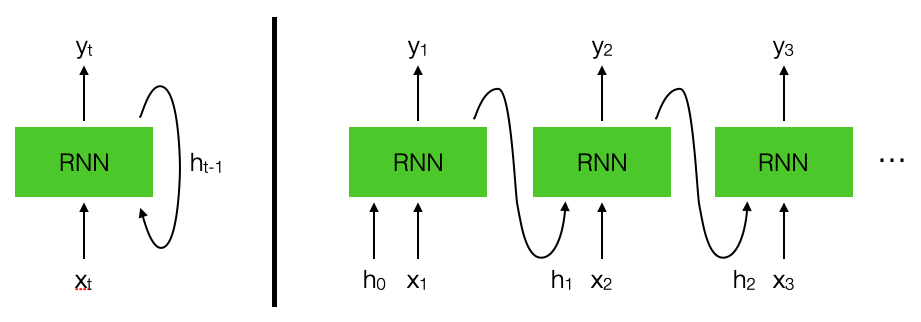
\includegraphics[width=\linewidth]{Images/ML/RNN.png}
    \caption{A standard recurrent neural net, shown in condensed form on the left, and in expanded form on the right. This net takes inputs $x_i$ and provides outputs $y_i$. A hidden state $h_i$ is retained in the net and passed back to the beginning after each input step.}
    \label{fig:RNN}
\end{figure}

The actual body of the RNN can be a neural net of any architecture, but in a standard RNN we typically use a simple few-layer densely connected net. The hidden state and output also typically pass through a $\tanh$ layer, with the output passing through an additional softmax layer. In this case, if we write the $\tanh$ function as $\sigma$, the concatenation of $x_t$ and $h_{t-1}$ as $x_t \oplus h_{t-1}$, and the neural net weight matrix as $W$, we can represent the RNN via the following equations:

\begin{align}
    o_t\oplus h_t&=\sigma(W(x_t\oplus h_{t-1})) \\
    y_t&=\text{softmax}(o_t)
\end{align}

If we examine this equation, we can see a problem which commonly comes up when training an RNN via gradient descent. We see that the final output $y_n$ depends on $W$, $x_n$, and $h_{n-1}$. But then $h_{n-1}$ further depends on $x_{n-1}$ and $h_{n-2}$, and so on. If we work out the full derivative of $y_n$ with respect to $W$, we get the following:

\begin{align}
    \frac{dy_n}{dW}&=\frac{\partial y_n}{\partial W} + \frac{\partial y_n}{\partial h_{n-1}}\frac{dh_{n-1}}{dW} \\
    &=\frac{\partial y_n}{\partial W} + \frac{\partial y_n}{\partial h_{n-1}}[\frac{\partial h_{n-1}}{\partial W} + \frac{\partial h_{n-1}}{\partial h_{n-2}}\frac{dh_{n-2}}{dW}] \\
    &=\frac{\partial y_n}{\partial W} + \frac{\partial y_n}{\partial h_{n-1}}[\frac{\partial h_{n-1}}{\partial W} + \frac{\partial h_{n-1}}{\partial h_{n-2}}[
    \frac{\partial h_{n-2}}{\partial W} + \frac{\partial h_{n-2}}{\partial h_{n-3}}\frac{dh_{n-3}}{dW}
    ]] \\
    &=... \nonumber
\end{align}

We then see that for all $t$:

\begin{align}
    \frac{\partial h_t}{\partial h_{t-1}} &= \sigma'(W(x_t\oplus h_{t-1}))W \\
    \frac{\partial h_t}{\partial W} &= \sigma'(W(x_t\oplus h_{t-1}))(x_t\oplus h_{t-1}) \\
    \frac{dy_n}{dW} &\approx \sum_{t=1}^{n} [\sigma'(W(x_t\oplus h_{t-1}))]^{n+1-t}W^{n-t}(x_t\oplus h_{t-1})
\end{align}

Since the derivative of $\sigma(x)$ quickly approaches zero as $x$ becomes non-zero, we see that terms with low values of $t$ essentially become irrelevant to training. In other words, the basic RNN has trouble learning long-range dependencies, and will in a sense "forget" the beginning of a sequence by the time it has calculated the final output. This behavior is called the vanishing gradient problem. In the case that W is large enough to overcome $\sigma'(x)$, we have the exploding gradient problem instead, but this issue is less common.

\section{LSTM and GRU}

<LSTM>

<GRU>

\section{Deep Sets}

\section{Transformers}